\section{Results}\label{sec:results}

\begin{comment}
This section should detail the obtained results in a clear,
easy-to-follow manner. It is important to make clear what are original
results and what are repeats of previous calculations or computations.
Remember that long tables of numbers are just as boring to read as
they are to type-in!

Use graphs to present your results wherever practicable.

Results or computations should be presented with uncertainties
(errors), both statistical and systematic where applicable.

Be selective in what you include: half a dozen \emph{e.g.}~tables that
contain wrong data you collected while you forgot to switch on the
computer are not relevant and may mask the correct results.
\end{comment}

\subsection{Radar Data Fit}\label{subsec:radardatafit}

%  TODO insert return chart
\begin{figure}[H]
    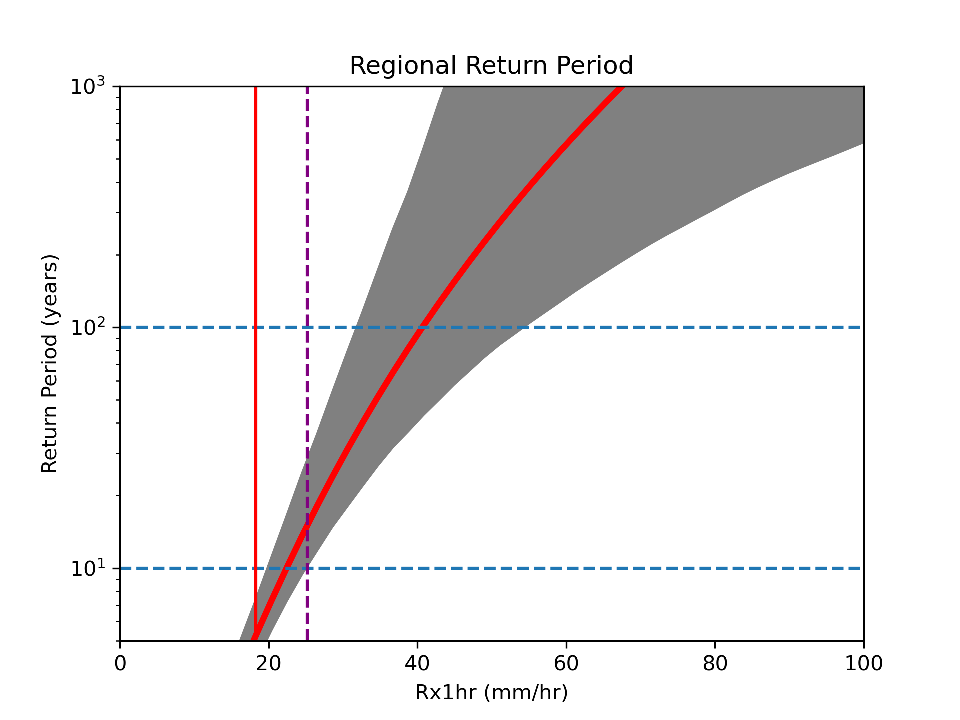
\includegraphics{radarreturnplot}
    \caption{A line graph plotting the return period in years against the magnitude of the event,
        taken from fitting a GEV distribution to the event distribution.
    The dashed purple vertical line is the magnitude of the Stonehaven event.
    The solid red vertical line is the actual one-hour rainfall maximum at the Stonehaven crash location.
    The grey area gives the uncertainties from a Monte Carlo bootstrap of ~1000 samples.}
    \label{fig:radarreturnplot}
\end{figure}

It was found that the maximum hourly rainfall at the crash location was 18.2mm/hr and
    that the empirical return period for the Stonehaven event was 17 years,
    as can be seen in figure~\ref{fig:radarreturnplot}.
The magnitude of the Stonehaven event,
    the 0.95 quantile of the radar grid cells having their 2020 seasonal maxima in the AM of the 12th of August,
    was found to be 25.2mm/hr.

Figure~\ref{fig:radarreturnplot} was created using the survival function of the GEV distribution fitted to the event data.
This had parameters location $\mu = 10.7$, scale $\sigma = 4.26$ and shape $\xi = -0.173$.

\subsection{Model Data}\label{subsec:modelcorr}

\subsubsection{Model Correlations}

\begin{figure}[H]
    \centering
    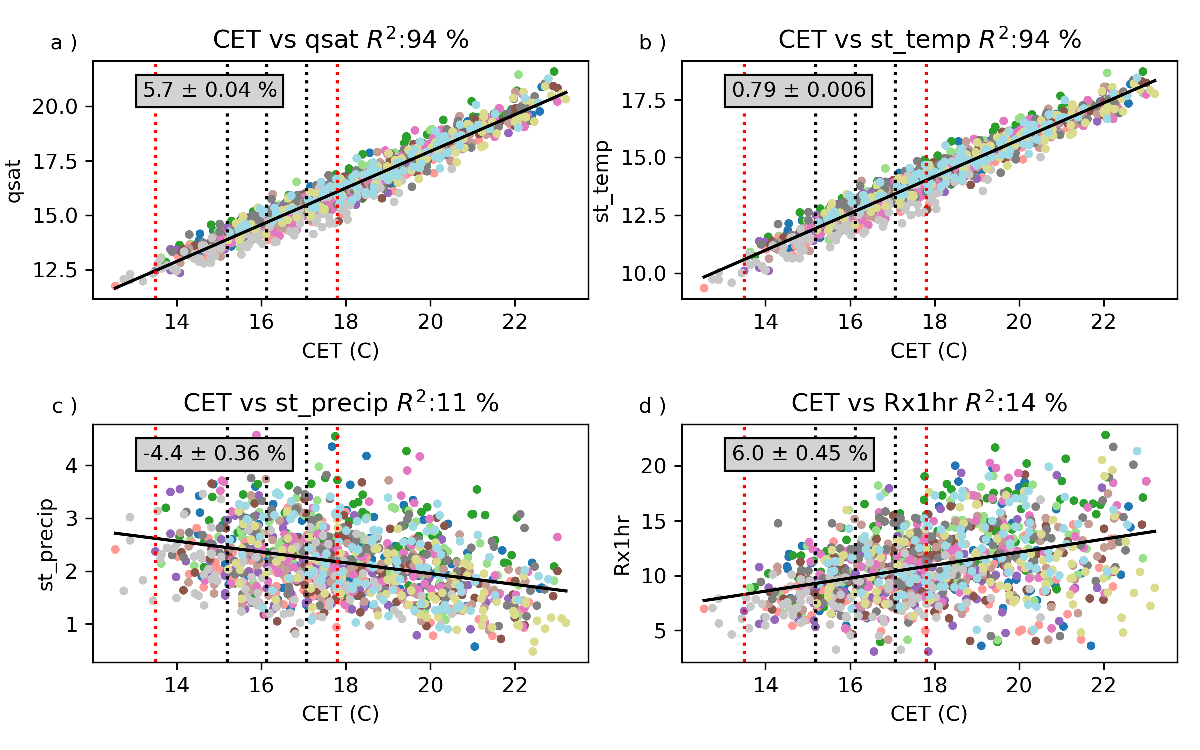
\includegraphics[width=150mm]{2cet_scatter}
    \caption{Scatter diagrams, from the Convection Permitting Model,
        for summer CET vs Edinburgh region saturated humidity (g/Kg) (a),
        Regional Temperature (b),
        Regional  Precipitation (mm/day) (c) and
        spatial median Rx1hr (mm/hr) for the region.
    The region is all points within a square of about 100x100km centered on the Stonehaven crash location.
    Colors indicate the ensemble number, black line is the best-fit regression slope.
    Text box shows best estimate and standard error in the estimated regression.
    Dotted black vertical lines show (left to right) CET summer mean for 1850--1899, 2021 and estimated CET at +2K warming.
    Title shows $R^2$ correlation coefficients for fit.
    Dotted vertical red lines show minimum and maximum CET values from 1850--2020 observations.}
    \label{fig:2cet_scatter}
\end{figure}

\subsubsection{Model GEV fit}

\begin{figure}[H]
    \centering
    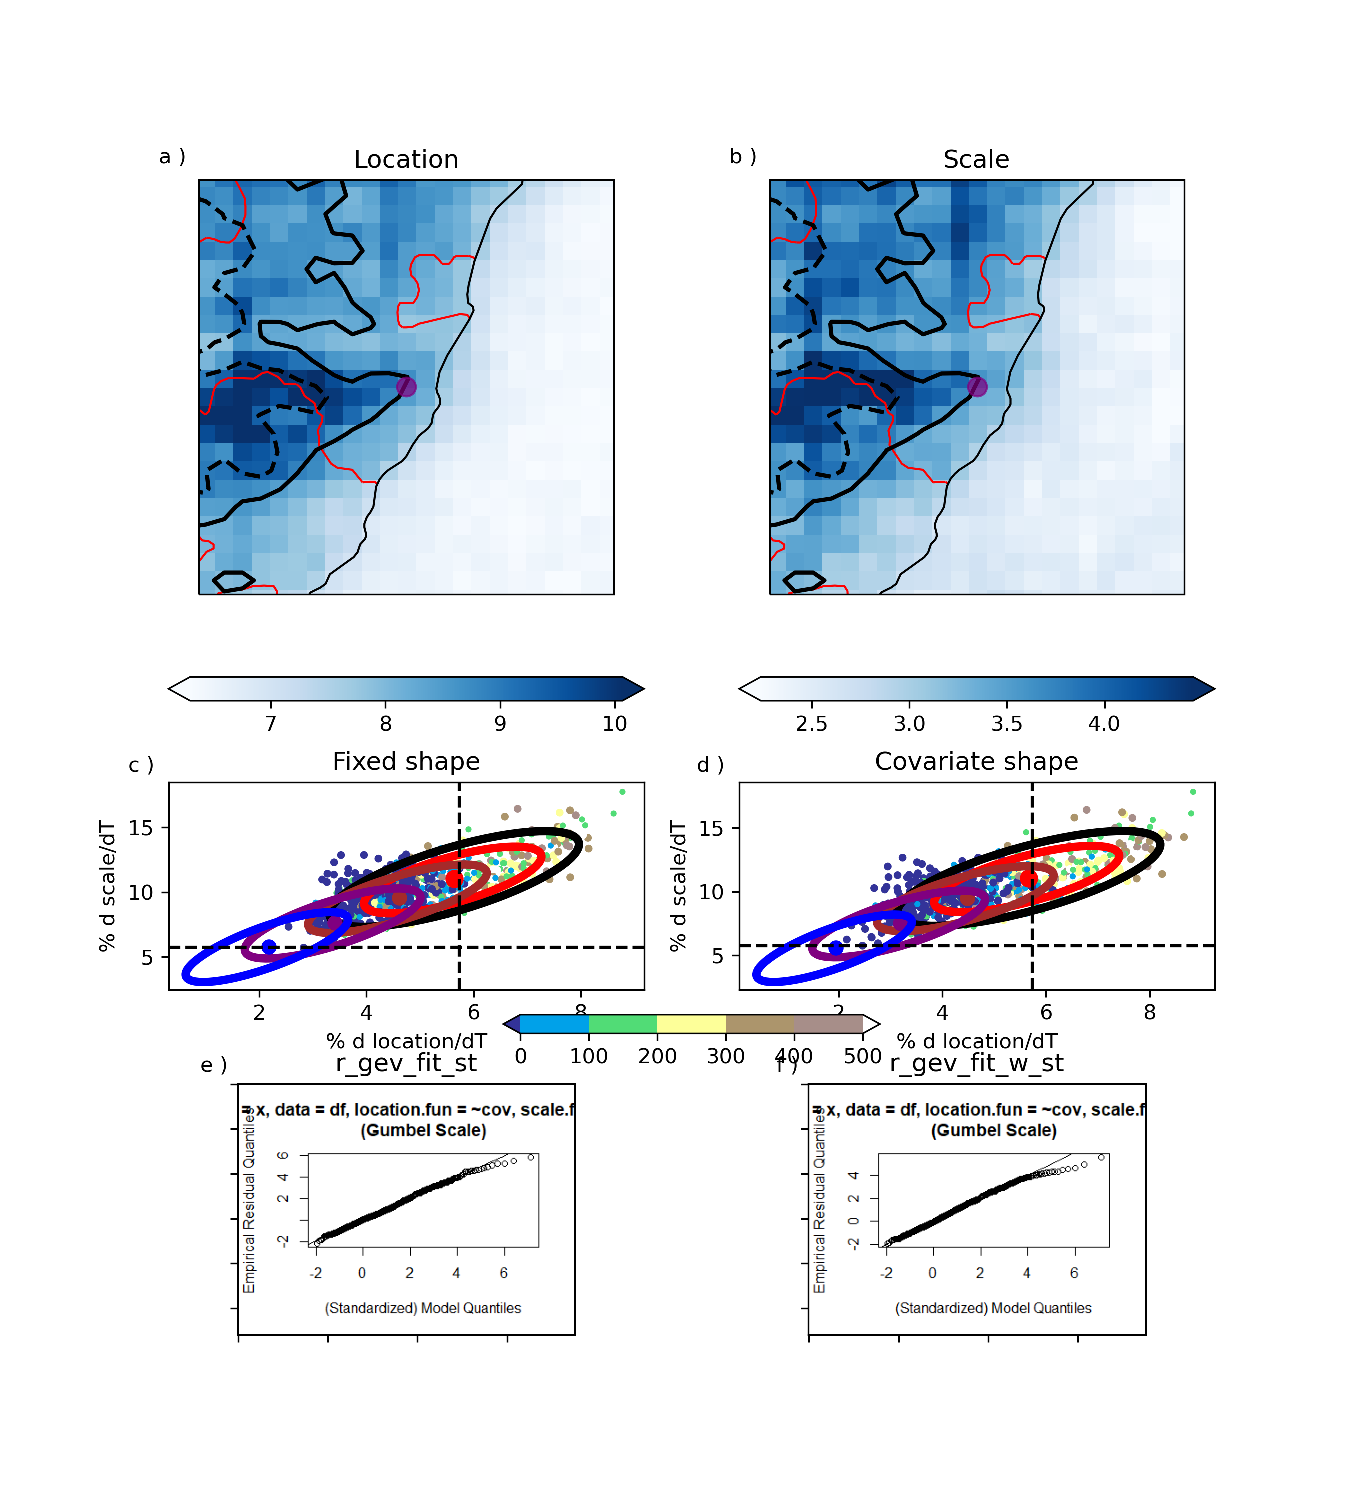
\includegraphics[width=100mm]{2cpm_gev_fit}
    \caption{a) Location parameter $\mu = \mu_0 + \overline{T_{2012-2021}}\mu_1$  for 2012--2021 CET and Rx1hr.
    b) Scale parameter $\sigma = \sigma_0 + \overline{T_{2012-2021}}\sigma_1$ for 2012--2021 CET and Rx1hr.
    c) Scatter plot of d(location)/d(CET) vs d(scale)/d(CET) as of 2012--2021 parameters.
    Dashed lines show expected changes if changes predicted by Clausius-Clapeyron relationship.
    Dots are colored by topography.
    Large red dot shows mean over all points where height is more than 0m and less than 400m.
    Red ellipse shows 95\% uncertainty for this mean assuming 1\% of data is independent (see methods).
    Other colored large dots and ellipses show similar means and uncertainty ellipses for Rx2hr (brown), Rx4hr (purple) and Rx8hr (blue).
    Black ellipse shows 95\% uncertainty for all Rx1hr points where height is less than 0m and more than 200m.
    d) as c) but for case with shape parameter varying with CET
    e) QQ-plot for GEV fit to CPM data using CET as a covariate at the Stonehaven Crash location.
    f) as d but for point 25km west of the Stonehaven Crash Location.}
    \label{fig:2cpm_gev_fit}
\end{figure}


\subsection{Risk Ratios}\label{subsec:riskratio}

%  TODO insert prob_radar_CPM

%  TODO insert plot showing overlap of distributions w/ parameters

\section{Discussion}\label{sec:discussion}

\begin{comment}
This section should give a picture of what you have taken out of your
project and how you can put it into context.

This section should summarise the results obtained, detail conclusions
reached, suggest future work, and changes that you would make if you
repeated the project.
\end{comment}

\subsection{Event Definition}\label{subsec:diseventdef}

%  TODO mention lack of trend analysis due to lack of radar data

%  TODO mention Koppen in analysis

\subsection{Model Resolution}\label{subsec:dismodeldef}

Mention~\cite{Kendon_Fischer_Short_2023}
%  TODO insert chart w various coarsenings

\subsection{Model Validity}\label{subsec:dismodelvalid}